\chapter{Analisi Associativa}
\label{ch:ass}

Di seguito verrà descritto il lavoro svolto nell'ambito della ricerca di regole associative. \\

Come è già stato accennato in precedenza, questo tipo di analisi ha richiesto l'impiego delle versioni discretizzate dei data set provenienti dalla fase di \textit{preprocessing}. Il motivo di questo requisito apparirà chiaro andando a descrivere brevemente il funzionamento delle tecniche di analisi associativa.

\section{Introduzione all'analisi associativa}

    Questa introduzione vuole essere solo un breve riassunto dei concetti fondamentali seguiti per realizzare all'atto pratico l'analisi. Una trattazione più approfondita --- che trascenderebbe  ampiamente lo scopo di questa tesi di laurea --- può essere trovata in \cite{dispense}, ed è proprio quella che è stata consultata per realizzare quanto segue.

    \subsection{Regole Associative}

        Una regola associativa è una implicazione del tipo $A \rightarrow B$, con $A$ e $B$ insiemi di item (detti, appunto \textit{itemset}). Il significato di ciò dovrebbe essere palese: data la presenza di $A$ in una istanza del data set, è \textit{fortemente probabile} la presenza di $B$. La valutazione di questa probabilità avviene considerando alcune metriche particolari quali, ad esempio, la \textit{confidenza} o il \textit{lift}. \\

        Portando un esempio sul data set oggetto di questa analisi, una tanto probabile quanto banale regola associativa che ci si aspetta di trovare potrà essere del tipo \textit{"Valutazione del corso: ALTA"} $\rightarrow$ \textit{"Voto conseguito: ALTO"}. \\

        Quello a cui si mira, però, è riuscire a scoprire qualche altra regola che trascenda il limite dell'ovvio, aprendo così le porte a interpretazioni non immediate dell'insieme di dati su cui si sta lavorando. Per questo motivo, oltre all'aiuto di criteri algoritmici di potatura, occorrerà comunque prevedere un \textit{intervento umano} nel \textit{post processing} delle regole generate.

    \subsection{L'algoritmo Apriori di Weka}
    \label{apriori}

    \begin{figure}
        \centering
        \caption{pannello di scelta delle impostazioni per l'algoritmo Apriori di Weka}
        \label{apriori_weka}
	    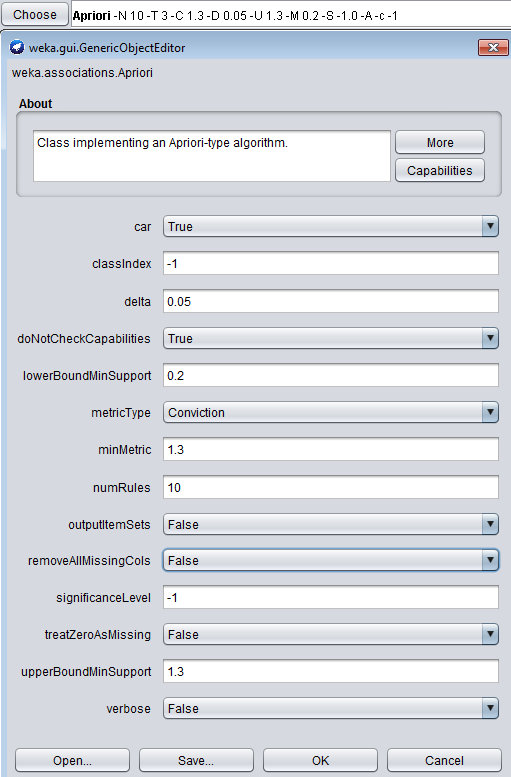
\includegraphics[scale=1.0]{img/apriori_weka.png}
    \end{figure}

        Il processo di generazione delle regole associative utilizzato in questa analisi si basa sul \textbf{principio Apriori}. Dato che una regola non è altro che una implicazione generata da un partizionamento binario di un itemset frequente, il pilastro fondamentale da cui partire per generare le regole è il \textit{mining} degli itemset frequenti. \\

        In estrema sintesi, l'idea generale è quella di generare una lista di \textit{candidati} semplici --- cioè di itemset che potrebbero essere frequenti --- verificarne il \textit{supporto} e usare quelli idonei per generare altri candidati più complessi. Il principio Apriori, infatti, stabilisce che se un itemset con pochi elementi è infrequente, lo saranno anche tutti gli itemset che lo comprendono. Questo fatto, detto \textit{anti-motonia} del supporto, ci consente di evitare di generare e calcolare la frequenza di ogni possibile itemset, rendendo trattabile quello che sarebbe invece un problema $NP-Completo$. \\

        Nel dettaglio dell'analisi da effettuare, l'algoritmo Apriori messo a disposizione dal software Weka accetta in input diversi parametri, che consentono di specificarne il comportamento dell'algoritmo, adattandolo agli scopi che ci si è prefissi. Si veda adesso una configurazione di esempio:\\

        \begin{center}
            \noindent \texttt{Apriori -N 10 -T 0 -C 0.9 -D 0.05 -U 1.0 -M 0.1}
        \end{center}

        I vari \textit{flags} da passare come argomenti vanno a regolare questi parametri della computazione:

        \begin{itemize}
            \item \texttt{-N}: numero di regole associative da trovare;
            \item \texttt{-T}: tipo di metrica utilizzata per la valutazione degli itemset
                \subitem 0 - \textit{confidence}
                \subitem 1 - \textit{lift}
                \subitem 2 - \textit{leverage}
                \subitem 3 - \textit{conviction};
            \item \texttt{-C}: valore minimo della metrica indicata per considerare frequente un itemset;
            \item \texttt{-D}: valore che viene usato per diminuire il supporto ad ogni iterazione dell'algoritmo;
            \item \texttt{-U}: limite superiore del supporto minimo richiesto;
            \item \texttt{-M}: limite inferiore del supporto minimo richiesto.
        \end{itemize}

        Ovviamente, come si può vedere in Figura \ref{apriori_weka}, sono possibili molte altre personalizzazioni e impostazioni, fatto che rende l'implementazione di Weka dell'algoritmo Apriori estremamente flessibile ed adattabile a molte esigenze. \\

\section{Apriori su dataset aggregato}

    Decidere a priori i parametri ottimali per l'algoritmo Apriori\footnote{gioco di parole \textbf{non} intenzionale.} è da considerarsi impossibile. Pertanto, anche in questo caso l'iter più adatto per ottenere dei risultati che possono essere giudicati interessanti è il banale ma efficace \textit{trial-and-error}. \\

    La conseguenza immediata di questo è che, similarmente a quanto fatto per la descrizione di altri tipi di analisi sui dati, in questa sezione verranno riportati solo gli output giudicati in qualche senso significativi. \\

    In ogni caso, alcune scelte sono state comuni a tutte le analisi:

    \begin{itemize}
        \item come \textit{metrica} è stato scelto il \textbf{Lift}, un cui valore positivo indica una correlazione effettiva --- cosa che non è affatto garantita da un alto valore di \textit{confidenza};
        \item non è stata usata la valutazione per classe, né il pruning per livello di significato;
        \item sono stati sempre stampati gli itemset frequenti, in quanto utili per capire l'andamento della generazione delle regole;
        \item come \textit{delta} è stato scelto un valore il più piccolo possibile, ma compatibile con dei tempi macchina "umani".
    \end{itemize}

        \subsection{Focus sul corso}

            L'analisi che viene presentata nel'immediato seguito è stata ottenuta cercando correlazioni fra gli attributi relativi all'andamento generale dei corsi d'esame. In particolare, oltre che verificare, come ipotizzato, la presenza di regole del tipo \textit{"Valutazione del corso: ALTA"} $\rightarrow$ \textit{"Voto conseguito: ALTO"}, andare a vedere se esistono legami fra questi due aspetti e il ritardo con cui uno studente supera un esame. \\

            L'algoritmo è stato lanciato sul data set \texttt{min\_d.csv}, ulteriormente semplificato grazie alla considerazione di questi soli attributi:

            \begin{itemize}
                \item identificativo dell'insegnamento;
                \item ritardo medio del superamento dell'esame (rispetto al primo appello disponibile, contato in semestri);
                \item voto medio ottenuto all'esame dagli studenti;
                \item valutazione media del corso d'insegnamento.
            \end{itemize}

            Il miglior risultato che si è ottenuto in quest'ottica è il seguente: \\

            \lstinputlisting{../ass/apriori_min_1.txt}

            \begin{figure}
                \centering
                \caption{visualizzazione 3D delle regole assciative trovate con focus sul corso}
                \label{apriori_min_1}
	            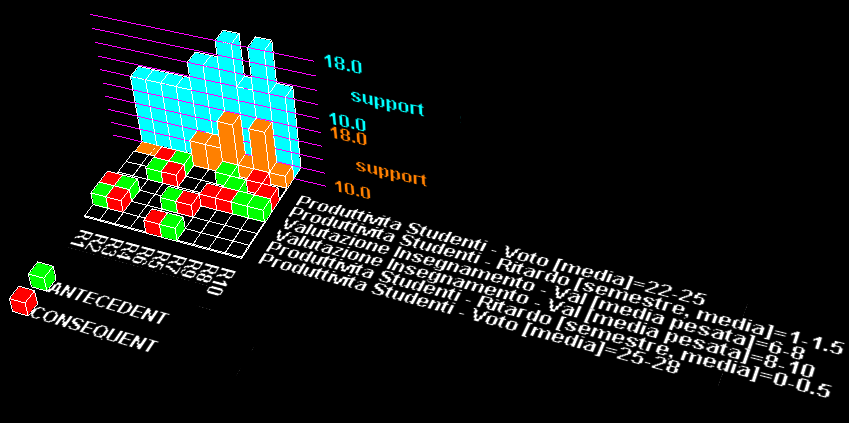
\includegraphics[scale=0.48]{../ass/apriori_min_1.png}
            \end{figure}

            Semplificando la \textit{naming convention} a favore della leggibilità, le regole trovate sono queste:

            \begin{itemize}
                \item \textbf{R1}: Ritardo: $BASSO$ $\rightarrow$ Valutazione insegnamento: $OTTIMA$
                \item \textbf{R2}: Valutazione insegnamento: $OTTIMA$ $\rightarrow$ Ritardo: $BASSO$
                \item \textbf{R3}: Ritardo: $ALTO$ $\rightarrow$ Voto: $MEDIO-BASSO$
                \item \textbf{R4}: Voto: $MEDIO-BASSO$ $\rightarrow$ Ritardo: $ALTO$
                \item \textbf{R5}: Voto: $MEDIO-ALTO$ $\rightarrow$ Valutazione insegnamento: $OTTIMA$
                \item \textbf{R6}: Valutazione insegnamento: $OTTIMA$ $\rightarrow$ Voto: $MEDIO-ALTO$
                \item \textbf{R7}: Voto: $MEDIO-BASSO$ $\rightarrow$ Valutazione insegnamenti: $SUFF.$
                \item \textbf{R8}: Valutazione insegnamenti: $SUFF.$ $\rightarrow$ Voto: $MEDIO-BASSO$
                \item \textbf{R9}: Ritardo: $ALTO$ $\rightarrow$ Valutazione insegnamenti: $SUFF.$
                \item \textbf{R10}: Valutazione insegnamenti: $SUFF.$ $\rightarrow$ Ritardo: $ALTO$
            \end{itemize}

            Andando ad analizzare le regole trovate, eliminando ridondanze ed effettuando una sorta di \textit{post processing} manualmente, le informazioni chiave che si sono ottenute risultano essere le seguenti:

            \begin{itemize}
                \item Ritardo: $BASSO$ $\leftarrow \rightarrow$ Valutazione insegnamento: $OTTIMA$
                \item Ritardo: $ALTO$ $\leftarrow \rightarrow$ Voto: $MEDIO-BASSO$
                \item Ritardo: $ALTO$ $\leftarrow \rightarrow$ Valutazione insegnamenti: $SUFF.$
                \item Voto: $MEDIO-ALTO$ $\leftarrow \rightarrow$ Valutazione insegnamento: $OTTIMA$
                \item Voto: $MEDIO-BASSO$ $\leftarrow \rightarrow$ Valutazione insegnamenti: $SUFF.$
            \end{itemize}

            Quelle trovate sono \underline{tutte} implicazioni doppie, il che significa che fra gli attributi esiste una forte correlazione. Messa da parte l'attesa e apparente proporzionalità diretta fra la valutazione del corso e il voto ottenuto all'esame, si può notare l'esistenza di una analoga correlazione fra il ritardo con cui gli studenti hanno superato l'esame e la valutazione del corso.

        \subsection{Focus sul docente}

            Facendo uso di alcuni, specifici attributi del dataset \texttt{full\_d.csv}, si è tentato di scoprire correlazioni fra la produttività degli studenti e l'aspetto della valutazione del corso relativo al docente. Nel particolare, sono stati considerati questi attributi:

            \begin{itemize}
                \item Identificativo del docente
                \item Ritardo medio del superamento dell'esame
                \item Voto medio ottenuto all'esame dagli studenti
                \item Valutazione media del paragrafo relativo al docente
            \end{itemize}

            Il miglior risultato che si è ottenuto, a seguito di iterazioni volte a proseguire nella direzione sopra descritta, è il seguente: \\

            \lstinputlisting{../ass/apriori_min_2.txt}

            \begin{figure}
                \centering
                \caption{visualizzazione 3D delle regole assciative trovate con focus sul docente}
                \label{apriori_min_2}
	            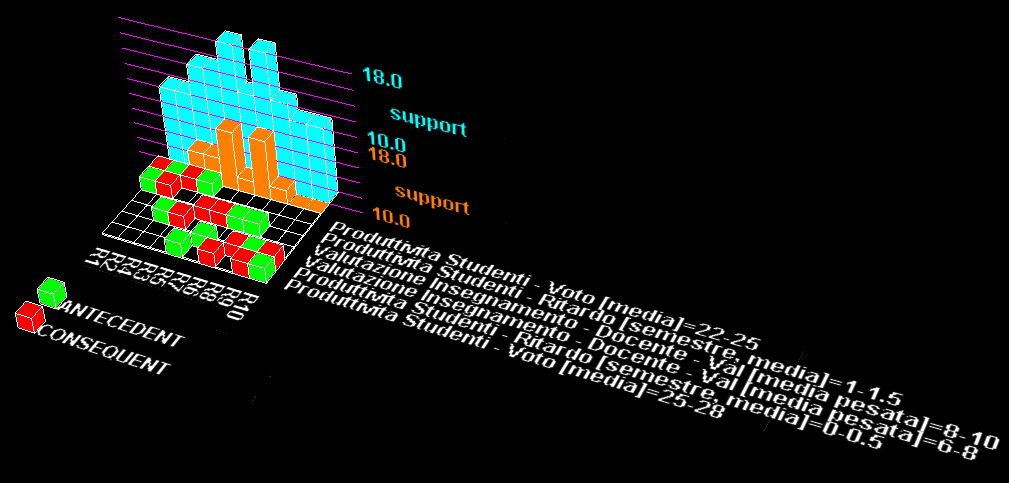
\includegraphics[scale=0.4]{../ass/apriori_min_2.png}
            \end{figure}

            Scartando immediatamente le regole già ottenute nell'analisi precedente --- quelle relative alle correlazioni fra il ritardo nel superamento e il voto all'esame --- si consideri la seguente sintesi delle regole trovate:

            \begin{itemize}
                \item Voto medio-basso $\leftarrow \rightarrow$ Valutazione docente sufficiente
                \item Voto medio-alto $\leftarrow \rightarrow$ Valutazione docente ottima
                \item Ritardo basso $\leftarrow \rightarrow$ Valutazione docente ottima
            \end{itemize}

            La correlazione fra la valutazione del docente e i risultati ottenuti appare molto forte, ma purtroppo è anche del tutto analoga a quella fra i risultati e la valutazione generale del corso.

        \subsection{Focus sulla Deviazione Standard}

        Nel data set \texttt{min\_d.csv} sono state mantenute informazioni complementari rispetto alle medie pesate dei valori che hanno composto l'aggregazione, quali ad esempio lo scarto quadratico medio di un certo attributo. Gli attributi contenenti questi dati sono stati ignorati nelle due precedenti analisi associative, pertanto è sembrato interessante vedere se esiste una qualche regola fra i seguenti parametri:

            \begin{itemize}
                \item Hash del docente
                \item Identificativo dell'insegnamento
                \item Percentuale di studenti il cui ritardo nel dare un certo esame supera il semestre
                \item Percentuale di studenti il cui voto conseguito in un dato esame supera il 24
                \item Deviazione standard dei voti ottenuti dagli studenti in quell'esame
                \item Media delle deviazioni standard delle valutazioni dell'insegnamento nei vari paragrafi
                \item Media delle percentuali di valutazioni dell'insegnamento sufficienti  
            \end{itemize}

            \lstinputlisting{../ass/apriori_min_3.txt}

            Non ci si aspettava di trovare niente di particolarmente significativo riguardo questi aspetti del data set. Invece, sono comparse due regole associative che possiamo riassumere in una implicazione doppia come segue:

            \begin{center}
                Deviazione standard del voto: MOLTO GRANDE $\leftarrow \rightarrow$ Deviazione standard della valutazione dell'insegnamento: GRANDE
            \end{center}

            Si tratta di una associazione forte, in quanto le due regole che la compongono hanno entrambe una confidenza abbastanza elevata --- R1: 0.8, R2: 0.68 --- ed un valore del lift sì minimo, ma comunque positivo. \\
